\documentclass[12pt,a4paper]{article}

%% ---------- mathematics ----------
\usepackage{amsmath,amsthm,amssymb,mathtools}

%% ---------- graphics & diagrams ----------
\usepackage{tikz}
\usetikzlibrary{arrows.meta,positioning,shapes.geometric,calc,fit,backgrounds,matrix,decorations.pathreplacing}
\usepackage{graphicx}

%% ---------- tables ----------
\usepackage{booktabs,tabularx,multirow,longtable,array}

%% ---------- algorithms ----------
\usepackage[ruled,vlined,linesnumbered]{algorithm2e}

%% ---------- coloured boxes ----------
\usepackage[most]{tcolorbox}

%% ---------- hyperlinks & cross-refs ----------
\usepackage{hyperref}
\usepackage[capitalize,noabbrev]{cleveref}

%% ---------- page layout ----------
\usepackage[margin=1in]{geometry}
\usepackage{fancyhdr}
\usepackage{enumitem}
\usepackage{xcolor}

%% ---------- fonts & misc ----------
\usepackage{microtype}

%% ============================================================
%%  Custom tcolorbox environments
%% ============================================================
\newtcolorbox{keyinsight}[1][]{%
  colback=blue!5!white,colframe=blue!75!black,
  fonttitle=\bfseries,title=Key Insight,#1}

\newtcolorbox{example}[1][]{%
  colback=green!5!white,colframe=green!75!black,
  fonttitle=\bfseries,title=Example,#1}

\newtcolorbox{warningbox}[1][]{%
  colback=red!5!white,colframe=red!75!black,
  fonttitle=\bfseries,title=Warning,#1}

%% ============================================================
%%  amsthm environments
%% ============================================================
\newtheorem{theorem}{Theorem}[section]
\newtheorem{lemma}[theorem]{Lemma}
\newtheorem{definition}{Definition}[section]
\newtheorem{remark}{Remark}[section]
\newtheorem{proposition}[theorem]{Proposition}
\newtheorem{corollary}[theorem]{Corollary}

%% ============================================================
%%  Custom commands (collected from all sessions in this file)
%% ============================================================
\newcommand{\tbf}[1]{\textbf{#1}}
\newcommand{\tit}[1]{\textit{#1}}
\newcommand{\ttt}[1]{\texttt{#1}}

\pagestyle{fancy}
\fancyhf{}
\lhead{\textsc{Deep Learning} --- IIIT Dharwad}
\rhead{Introduction, Course Plan, and PyTorch Foundations}
\rfoot{Page \thepage}
\lfoot{Prof.\ S R M Prasanna \& Dr.\ Sunil Saumya}
\renewcommand{\headrulewidth}{0.4pt}

\title{%
  {\Large\bfseries Deep Learning Course}\\[6pt]
  {\LARGE Introduction, Course Plan, and PyTorch Foundations}\\[4pt]
  {\normalsize IIIT Dharwad --- M.Tech Programme}
}
\author{Prof.\ S R M Prasanna \& Dr.\ Sunil Saumya}
\date{Sessions 1, 2}

\begin{document}

\maketitle
\tableofcontents
\clearpage

%% ============================================================
%% Session 01: Introduction, Course Plan, and Historical Foundations of Deep Learning
%% ============================================================
\part{Session 01: Introduction, Course Plan, and Historical Foundations of Deep Learning}

%% ============================================================

\begin{abstract}
These notes document Session~01 of the Deep Learning course offered at
IIIT Dharwad to M.Tech students across super-specialisations.  The session
serves as a course orientation and motivation lecture: it presents the
8-week course plan with PyTorch hands-on components, traces the history of
deep learning from the 2006 Hinton \emph{et al.}\ breakthrough, explains the
conceptual distinction between classical Machine Learning and Deep Learning,
and situates Deep Learning within the broader AI taxonomy
(AI~$\supset$~ML~$\supset$~NN~$\supset$~DL~$\supset$~GAI).  Mathematical
notation, TikZ diagrams, and structured summaries are included to aid
self-study.
\end{abstract}

\newpage

%% ============================================================
\section{Introduction}
\label{sec:intro}
%% ============================================================

Deep Learning is described by the instructors as a \emph{cornerstone course}
for Data Science and Artificial Intelligence.  The course is mandatory for all
M.Tech super-specialisations because modern intelligent systems — from
automatic speech recognition to large language models — rely on deep neural
architectures.

The primary pedagogical shift in this offering, compared to earlier editions of
the course, is the integration of \emph{hands-on PyTorch programming} alongside
each theory module.  As Prof.\ Prasanna explains in the lecture:

\begin{quote}
``Since you are all working professionals, we thought: how do we give
maximum benefit of this course?  Dr.\ Sunil suggested we make this course
more hands-on, such that once you complete it you also have exposure to open
source toolkits for training and testing deep learning models, which will be
useful from a career point of view.''
\end{quote}

\subsection{Session Objectives}
\label{subsec:objectives}

By the end of Session~01 the student should be able to:
\begin{enumerate}[label=\textbf{O\arabic*.}]
  \item Identify the eight-week syllabus structure and the corresponding
        hands-on PyTorch tasks.
  \item Describe the 2006 Hinton \emph{et al.}\ breakthrough and explain why
        it revived the deep learning field.
  \item Distinguish Classical Machine Learning from Deep Learning in terms
        of feature engineering.
  \item Situate Deep Learning within the AI~$\supset$~ML~$\supset$~NN~$\supset$~DL~$\supset$~GAI hierarchy.
  \item Appreciate the three enabling factors that made deep learning
        practical: (i) algorithmic advances, (ii) big data availability, and
        (iii) GPU computing power.
\end{enumerate}

\subsection{Course Metadata}
\label{subsec:metadata}

\begin{center}
\begin{tabular}{ll}
\toprule
\textbf{Item} & \textbf{Detail} \\
\midrule
Course name   & Deep Learning (3 Credits) \\
Semester      & Second Semester, M.Tech \\
Instructors   & Prof.\ S R M Prasanna; Dr.\ Sunil Saumya \\
Slide deck    & \texttt{01DLPlan} (21 slides) \\
Video         & \url{https://vimeo.com/1137772716} \\
Platform      & PyTorch (open-source) \\
Assessment    & Class notes 15\%; X-factor 10\%; Assignments 20\%;\\
              & Quiz 10\%; Mid-term; End-term (65\% written total) \\
\bottomrule
\end{tabular}
\end{center}

%% ============================================================
\section{Background and Prerequisites}
\label{sec:background}
%% ============================================================

\subsection{Recommended Reading}
\label{subsec:books}

The instructors provided the following reference list for students who wish to
go beyond the lecture slides.  These texts are \emph{supplementary}; the
slide decks and hands-on notebooks are self-sufficient for the course.

\begin{enumerate}[label=\arabic*.]
  \item R.\ O.\ Duda and P.\ E.\ Hart, \emph{Pattern Classification},
        Wiley, 2001.
  \item C.\ M.\ Bishop, \emph{Neural Networks for Pattern Recognition},
        Oxford University Press, 1995.
  \item B.\ Yegnanarayana, \emph{Artificial Neural Networks},
        PHI Learning, 1999.
  \item C.\ M.\ Bishop, \emph{Pattern Recognition and Machine Learning (PRML)},
        Springer, 2006.
  \item M.\ Nielsen, \emph{Neural Networks and Deep Learning} (open book,
        freely available online).
  \item I.\ Goodfellow \emph{et al.}, \emph{Deep Learning},
        MIT Press, 2016.
  \item C.\ C.\ Aggarwal, \emph{Neural Networks and Deep Learning},
        Springer, 2018.
  \item M.\ M.\ Khapra, \emph{Deep Learning Parts I \& II},
        NPTEL Course (IIT Madras).
  \item A.\ Ghodsi, \emph{Deep Learning},
        University of Waterloo (online lectures).
  \item C.\ M.\ Bishop and H.\ Bishop, \emph{Deep Learning},
        Springer, 2024.
\end{enumerate}

\begin{keyinsight}
Prof.\ Prasanna personally recommends the NPTEL course by Mithesh Khapra
(IIT Madras) and Ali Ghodsi's University of Waterloo course as complementary
online resources.  The 2024 Bishop \& Bishop text is also highlighted as the
most up-to-date reference on the subject.
\end{keyinsight}

\subsection{Mathematical Prerequisites}
\label{subsec:mathprereq}

Students are expected to be comfortable with the following:

\begin{itemize}
  \item \textbf{Linear algebra}: matrix multiplication, eigenvalues, norms.
  \item \textbf{Calculus}: partial differentiation, chain rule — essential for
        back-propagation.
  \item \textbf{Probability and statistics}: Bayes rule, Gaussian distributions,
        maximum-likelihood estimation.
  \item \textbf{Optimisation}: gradient descent, convexity, saddle points.
  \item \textbf{Programming}: Python fluency; basic familiarity with NumPy and
        Matplotlib.
\end{itemize}

The key mathematical relation underlying supervised learning is a functional
mapping:
\begin{equation}
  \label{eq:functional_mapping}
  \hat{y} = f(\mathbf{x};\,\boldsymbol{\theta}),
\end{equation}
where $\mathbf{x} \in \mathbb{R}^d$ is the input feature vector, $\hat{y}$ is
the predicted output, and $\boldsymbol{\theta}$ denotes all learnable
parameters.  The learning procedure minimises a loss:
\begin{equation}
  \label{eq:loss}
  \mathcal{L}(\boldsymbol{\theta})
  = \frac{1}{N}\sum_{i=1}^{N} \ell\!\left(y_i,\, f(\mathbf{x}_i;\boldsymbol{\theta})\right),
\end{equation}
where $\{(\mathbf{x}_i, y_i)\}_{i=1}^{N}$ is the training set and $\ell$ is a
per-sample loss function (e.g., cross-entropy for classification, mean-squared
error for regression).

%% ============================================================
\section{Course Structure and Syllabus}
\label{sec:courseplan}
%% ============================================================

The 8-week core curriculum is organised so that each session has a \emph{theory
component} (aligned with the official syllabus) and a \emph{hands-on component}
implemented in PyTorch.  \cref{tab:weeks12,tab:weeks34,tab:weeks58} reproduce
the three course-plan slides presented in the lecture.

\subsection{Weeks 1--2: Neural Networks Foundations}
\label{subsec:weeks12}

\begin{table}[ht]
\centering
\caption{Deep Learning Course Plan — Weeks 1--2 (Slide V03).}
\label{tab:weeks12}
\begin{tabularx}{\textwidth}{cclX}
\toprule
\textbf{Week} & \textbf{Session} & \textbf{Theory Topics} & \textbf{Hands-on (PyTorch)} \\
\midrule
1 & 1 & Biological vs.\ Artificial Neuron; Neural Networks; Learning Laws
      & Implement perceptron (logical gates) in PyTorch \\
\addlinespace
1 & 2 & Feedforward Networks; Backpropagation
      & Manual backprop; Build 2-layer NN in PyTorch \\
\addlinespace
2 & 3 & Deep Feedforward NNs; Training Deep Networks; Vanishing Gradients
      & Train deep MLP on MNIST \\
\addlinespace
2 & 4 & Greedy Layer-wise Training; Training Belief Networks; Practical Tricks
      & Layer-wise pre-training demo; effect of depth \\
\bottomrule
\end{tabularx}
\end{table}

\subsection{Weeks 3--4: Convolutional Neural Networks}
\label{subsec:weeks34}

\begin{table}[ht]
\centering
\caption{Deep Learning Course Plan — Weeks 3--4 (Slide V04).}
\label{tab:weeks34}
\begin{tabularx}{\textwidth}{cclX}
\toprule
\textbf{Week} & \textbf{Session} & \textbf{Theory Topics} & \textbf{Hands-on (PyTorch)} \\
\midrule
3 & 5 & CNN vs.\ Other NNs; Convolution Basics; Filters; Feature Maps
      & Manual convolution; visualising filters \\
\addlinespace
3 & 6 & CNN Modules: Pooling, Padding, Stride; CNN Training Pipeline
      & Train simple CNN \\
\addlinespace
4 & 7 & CNN as Feature Extractor; CNN as Classifier
      & Use pre-trained CNN for feature extraction \\
\addlinespace
4 & 8 & Significance of CNNs in Object Classification Tasks
      & Error analysis, confusion matrix, Grad-CAM \\
\bottomrule
\end{tabularx}
\end{table}

\subsection{Weeks 5--8: Sequence Models and Transformers}
\label{subsec:weeks58}

\begin{table}[ht]
\centering
\caption{Deep Learning Course Plan — Weeks 5--8 (Slide V05).}
\label{tab:weeks58}
\begin{tabularx}{\textwidth}{cclX}
\toprule
\textbf{Week} & \textbf{Session} & \textbf{Theory Topics} & \textbf{Hands-on (PyTorch)} \\
\midrule
5  &  9 & Sequence Models
       & Build simple RNN for sequence prediction \\
\addlinespace
5  & 10 & Recurrent Neural Networks (RNN): Architecture, BPTT
       & RNN-based character/word-level model \\
\addlinespace
6  & 11 & Long Short-Term Memory (LSTM) Networks
       & LSTM for sentiment analysis \\
\addlinespace
6  & 12 & Gated Recurrent Units (GRU)
       & Train GRU and compare with LSTM \\
\addlinespace
7  & 13 & Seq2Seq Models: Encoder--Decoder Architecture
       & Seq2Seq for toy translation / copying task \\
\addlinespace
7  & 14 & Attention Modelling: Bahdanau, Luong
       & Add attention to Seq2Seq model \\
\addlinespace
8  & 15 & Attention: Scaled Dot-Product, Multi-Head
       & Implement scaled dot-product attention \\
\addlinespace
8  & 16 & Transformers: Encoder/Decoder Architecture
       & Mini-transformer block implementation \\
\bottomrule
\end{tabularx}
\end{table}

\begin{keyinsight}
The progression follows a deliberate pedagogical arc:
\begin{center}
Perceptron $\;\longrightarrow\;$ Deep MLP $\;\longrightarrow\;$ CNN
$\;\longrightarrow\;$ RNN/LSTM $\;\longrightarrow\;$ Transformer
$\;\longrightarrow\;$ Generative Models.
\end{center}
Each transition introduces a new inductive bias suited to a different
problem structure (static feature vectors, spatial grids, temporal sequences,
long-range dependencies).
\end{keyinsight}

\subsection{Sequence-to-Sequence and Generative Models (Overview)}
\label{subsec:seq2gen}

After Week~8, the course extends to:
\begin{itemize}
  \item \textbf{Weeks 9--10}: Transformers in detail — architecture, training,
        applications (machine translation, question answering, named entity
        recognition).
  \item \textbf{Weeks 11--13}: Generative models — Variational Autoencoders
        (VAEs), Generative Adversarial Networks (GANs), Generative Pre-trained
        Transformer (GPT).
  \item \textbf{Week 14}: Advanced topics and extended code demonstrations
        (time-permitting).
\end{itemize}

The key concept underpinning sequence-to-sequence learning is the
\emph{encoder--decoder} formulation.  Given an input sequence
$\mathbf{x} = (x_1, x_2, \ldots, x_T)$, the encoder maps it to a fixed-length
context vector $\mathbf{c}$:
\begin{equation}
  \label{eq:encoder}
  \mathbf{c} = \mathrm{Enc}(x_1, \ldots, x_T;\,\boldsymbol{\theta}_\mathrm{enc}),
\end{equation}
and the decoder generates the output sequence
$\mathbf{y} = (y_1, y_2, \ldots, y_{T'})$ one token at a time:
\begin{equation}
  \label{eq:decoder}
  P(y_t \mid y_1,\ldots,y_{t-1},\,\mathbf{c};\,\boldsymbol{\theta}_\mathrm{dec}).
\end{equation}

%% ============================================================
\section{History of Deep Learning}
\label{sec:history}
%% ============================================================

\subsection{The Neural Network Era (Pre-2006)}
\label{subsec:pre2006}

The intellectual lineage of deep learning traces back to artificial neural
networks inspired by the structure and functioning of the human brain.  The
brain achieves its remarkable cognitive power not through a single neuron, but
through \emph{billions of neurons} working in a loosely connected,
parallel, and distributed fashion.  Early researchers sought to mimic this
\emph{parallel and distributed processing} on digital computers.

\begin{definition}[Artificial Neural Network]
\label{def:ann}
An \emph{Artificial Neural Network} (ANN) is a parameterised, layered
computational graph of artificial neurons, each computing a non-linear
function of a weighted sum of its inputs.  Formally, the output of neuron $j$
in layer $l$ is:
\begin{equation}
  \label{eq:neuron}
  a_j^{(l)} = \phi\!\left(\sum_{k} w_{jk}^{(l)}\, a_k^{(l-1)} + b_j^{(l)}\right),
\end{equation}
where $w_{jk}^{(l)}$ are synaptic weights, $b_j^{(l)}$ is a bias,
and $\phi(\cdot)$ is an activation function.
\end{definition}

Shallow neural networks (1--2 hidden layers) emerged as an alternative
computing model for classical machine learning tasks.  They were trained using
the \emph{Back-Propagation} (BP) algorithm, which applies the chain rule to
compute gradients of the loss with respect to all parameters:
\begin{align}
  \label{eq:backprop}
  \frac{\partial \mathcal{L}}{\partial w_{jk}^{(l)}}
  &= \frac{\partial \mathcal{L}}{\partial a_j^{(l)}}
     \cdot \phi'\!\left(z_j^{(l)}\right)
     \cdot a_k^{(l-1)},
\end{align}
where $z_j^{(l)} = \sum_k w_{jk}^{(l)} a_k^{(l-1)} + b_j^{(l)}$ is the
pre-activation.

Despite theoretical appeal, shallow networks could not consistently outperform
classical machine learning methods (SVMs, GMMs, decision trees) on many
benchmarks.  This led researchers to hypothesise that \emph{deeper}
architectures — with more layers and more parameters — would capture richer
representations.

\subsection{The Dark Age: Vanishing Gradients and Insufficient Data}
\label{subsec:darkage}

Attempts to scale up neural networks to many layers ran into two fundamental
obstacles:

\begin{warningbox}
\textbf{Obstacle 1 — Vanishing Gradient Problem.}
When back-propagating through many layers, the gradient signal is multiplied
by the weight matrix and the derivative of the activation function at each
step.  For activations such as the sigmoid $\sigma(z) = 1/(1+e^{-z})$, the
derivative $\sigma'(z) = \sigma(z)(1-\sigma(z)) \leq 0.25$ at all points.
Through $L$ layers, the gradient can shrink exponentially:
\begin{equation}
  \label{eq:vanishing}
  \left\|\frac{\partial \mathcal{L}}{\partial \mathbf{W}^{(1)}}\right\|
  \;\propto\; \prod_{l=2}^{L} \left\|\mathbf{W}^{(l)}\right\|
              \prod_{l=2}^{L} \left|\sigma'\!\left(z^{(l)}\right)\right|
  \;\longrightarrow\; 0 \quad \text{as } L \to \infty.
\end{equation}
Parameters in early layers receive almost no gradient signal and fail to learn.

\textbf{Obstacle 2 — Insufficient Training Data.}
In the 1990s and early 2000s, labelled datasets were small by modern
standards.  A large deep network trained on insufficient data
\emph{over-fits}: it memorises the training examples and fails to generalise
to new inputs.
\end{warningbox}

As a result, most of the research community abandoned deep architectures in
the late 1990s.

\subsection{The 2006 Breakthrough: Hinton \emph{et al.}}
\label{subsec:hinton2006}

A small group of researchers — led by Geoffrey Hinton at the University of
Toronto, who later received both the Turing Award and the Nobel Prize in
Physics for this work — continued to pursue deep architectures through the
early 2000s.  In 2006 they published a landmark paper:

\begin{quote}
Geoffrey E.\ Hinton, Simon Osindero, and Yee-Whye Teh,
``A Fast Learning Algorithm for Deep Belief Nets,''
\emph{Neural Computation}, vol.\ 18, pp.\ 1527--1554, 2006.
\end{quote}

\begin{keyinsight}[title=The 2006 Breakthrough]
Hinton \emph{et al.}\ introduced \emph{greedy layer-wise pre-training}:
each layer of a Deep Belief Network (DBN) is first trained unsupervised as a
Restricted Boltzmann Machine (RBM), using efficient contrastive divergence.
The pre-trained weights then serve as a good initialisation for fine-tuning
the entire network with back-propagation.  This strategy:
\begin{enumerate}
  \item Circumvented the vanishing gradient problem by initialising weights
        near a good solution.
  \item Achieved state-of-the-art accuracy ($>98\%$) on the MNIST handwritten
        digit recognition benchmark.
  \item Demonstrated that deep networks are trainable and outperform
        classical ML on real tasks.
\end{enumerate}
This paper gave deep learning its modern name and triggered a ``snowball
effect'' that, within a decade (2006--2016), led to deep learning conquering
industry benchmarks.
\end{keyinsight}

\subsection{The Three Enabling Factors (Post-2006)}
\label{subsec:enablers}

The instructor identifies three converging advances that made modern deep
learning possible:

\begin{enumerate}[label=\textbf{E\arabic*.}]
  \item \textbf{Algorithmic innovations}: greedy pre-training, ReLU
        activations, Dropout, Batch Normalisation, residual connections.
  \item \textbf{Big data}: the connected world generated vast labelled
        datasets (ImageNet, Common Crawl, LibriSpeech, etc.).
  \item \textbf{GPU computing}: graphics processors enabled massively parallel
        matrix multiplications, reducing training time from weeks to hours.
\end{enumerate}

\begin{remark}
\label{rem:timeline}
The snowball accelerated rapidly.  AlexNet (2012) won ImageNet with a
top-5 error of $15.3\%$, crushing the classical-vision runner-up at $26.2\%$.
By 2016 deep learning held state-of-the-art on image classification, speech
recognition, machine translation, and game-playing.  The introduction of the
Transformer architecture (Vaswani \emph{et al.}, 2017) and subsequent
large language models further accelerated the field into the Generative AI era.
\end{remark}

%% ============================================================
\section{Machine Learning vs.\ Deep Learning}
\label{sec:mldl}
%% ============================================================

\subsection{Classical Machine Learning Pipeline}
\label{subsec:classical_ml}

Classical (shallow) machine learning requires a \emph{domain expert} to
manually engineer features before training a model.  The pipeline is:

\begin{equation}
  \label{eq:ml_pipeline}
  \underbrace{\text{Raw Input}}_{\mathbf{x}_\mathrm{raw}}
  \xrightarrow{\text{Feature Engineering}}
  \underbrace{\text{Feature Vector}}_{\boldsymbol{\phi}(\mathbf{x})}
  \xrightarrow{\text{Classifier / Regressor}}
  \hat{y}.
\end{equation}

The feature engineering step encodes domain knowledge: for image data this
might be HOG descriptors or SIFT keypoints; for audio it might be MFCC
coefficients; for text it might be TF-IDF bag-of-words vectors.

\begin{example}[title=Spam Email Detection (Rule-Based vs.\ ML)]
\textbf{Rule-based}: A programmer explicitly lists keywords (``free'',
``prize'', ``winner'') and directs the program to flag emails containing
them.  The programmer tells the system exactly what to look for.

\textbf{Classical ML}: The engineer labels a set of emails as
\texttt{spam=1} or \texttt{spam=0} and extracts features (word frequency
vectors, sender domain, etc.).  A logistic regression or SVM learns the
decision boundary from data, without being told which words matter.

\textbf{Deep Learning}: Raw email text (or pixels, if image-based) is fed
directly to a deep network.  The network simultaneously discovers relevant
features \emph{and} learns the classification rule end-to-end.
\end{example}

\subsection{Deep Learning Pipeline}
\label{subsec:dl_pipeline}

Deep Learning eliminates the manual feature-engineering step:

\begin{equation}
  \label{eq:dl_pipeline}
  \underbrace{\text{Raw Input}}_{\mathbf{x}_\mathrm{raw}}
  \xrightarrow{\text{Deep Network (end-to-end)}}
  \hat{y}.
\end{equation}

The early layers of the network automatically learn low-level features
(edges, textures, phonemes), and progressively deeper layers combine them
into higher-level semantic representations.  This is the key distinction:

\begin{definition}[Deep Learning]
\label{def:deep_learning}
\emph{Deep Learning} is a subfield of machine learning that uses multi-layer
neural networks (typically $L \geq 3$ hidden layers) to learn hierarchical
representations directly from raw data, obviating manual feature engineering.
The learned representation at layer $l$ is:
\begin{align}
  \label{eq:hierarchical}
  \mathbf{h}^{(1)} &= \phi\!\left(\mathbf{W}^{(1)}\mathbf{x} + \mathbf{b}^{(1)}\right), \\
  \mathbf{h}^{(l)} &= \phi\!\left(\mathbf{W}^{(l)}\mathbf{h}^{(l-1)} + \mathbf{b}^{(l)}\right),
                    \quad l = 2,\ldots,L, \\
  \hat{y}          &= g\!\left(\mathbf{W}^{(L+1)}\mathbf{h}^{(L)} + \mathbf{b}^{(L+1)}\right),
\end{align}
where $g(\cdot)$ is the output activation (e.g., softmax for classification).
\end{definition}

\subsection{Comparison Table: Shallow NN vs.\ Deep Learning}
\label{subsec:comparison}

The following table is reproduced from Slide V08 of the lecture:

\begin{table}[ht]
\centering
\caption{Neural Networks (shallow) vs.\ Deep Learning --- key distinctions (Slide V08).}
\label{tab:nn_vs_dl}
\begin{tabularx}{\textwidth}{lXX}
\toprule
\textbf{Aspect} & \textbf{Neural Networks (Shallow)} & \textbf{Deep Learning} \\
\midrule
Depth & 1--2 hidden layers & Many hidden layers ($L \gg 2$) \\
\addlinespace
Training algorithm & Back-propagation works well & BP struggles; vanishing gradients \\
\addlinespace
Data requirement & Moderate dataset sufficient & Large datasets required \\
\addlinespace
Feature engineering & Manual features necessary & Automatic feature learning \\
\addlinespace
Model size & Small parameter count & Millions to billions of parameters \\
\addlinespace
Computational cost & Low (CPU-feasible) & High (GPU/TPU required) \\
\addlinespace
Representative models & Perceptron, MLP, SVM & CNN, LSTM, Transformer, GPT \\
\bottomrule
\end{tabularx}
\end{table}

\begin{keyinsight}
The fundamental reason shallow networks needed manual features is their
\emph{limited capacity}: with only 1--2 hidden layers, the model lacks the
representational power to discover complex hierarchical features itself.
Depth provides exponential representational advantage, a fact formalised
by the depth separation theorems in circuit complexity theory.
\end{keyinsight}

%% ============================================================
\section{The AI Taxonomy: AI $\supset$ ML $\supset$ NN $\supset$ DL $\supset$ GAI}
\label{sec:taxonomy}
%% ============================================================

\subsection{The Nested Hierarchy}
\label{subsec:nested}

The final slides of the session situate Deep Learning within the broader
intellectual landscape using a nested-circles diagram (Slide V10).

\begin{figure}[ht]
\centering
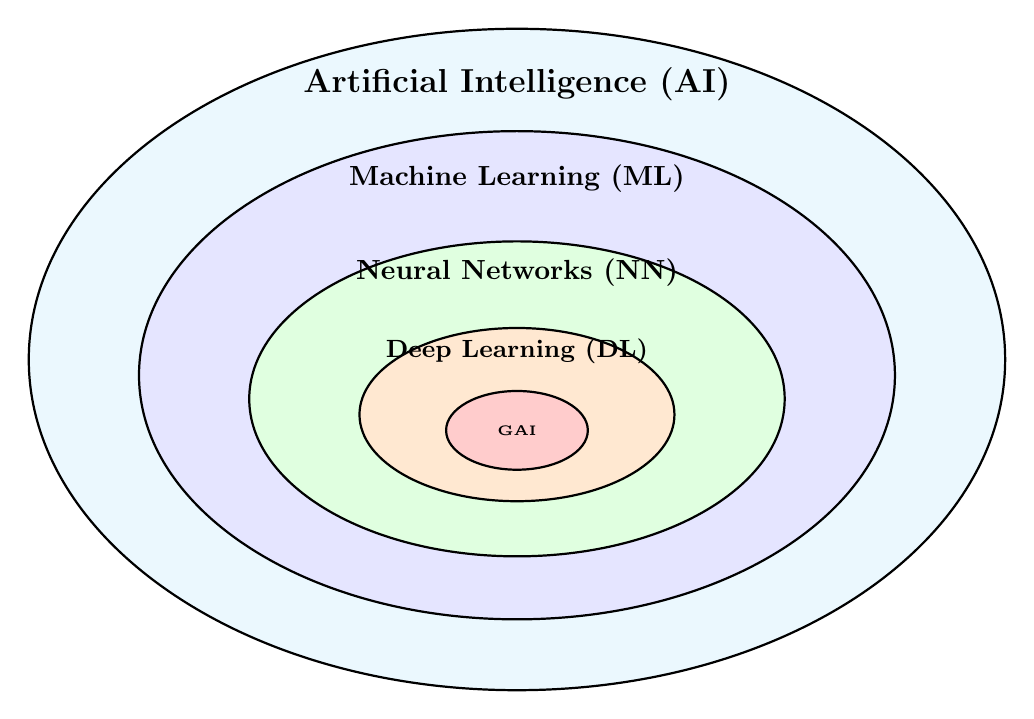
\begin{tikzpicture}[scale=1.0]
  %% Outermost: AI
  \draw[thick, fill=cyan!8]
    (0,0) ellipse (6.2cm and 4.2cm);
  \node[font=\large\bfseries] at (0,3.5) {Artificial Intelligence (AI)};

  %% ML
  \draw[thick, fill=blue!10]
    (0,-0.2) ellipse (4.8cm and 3.1cm);
  \node[font=\bfseries] at (0,2.3) {Machine Learning (ML)};

  %% NN
  \draw[thick, fill=green!12]
    (0,-0.5) ellipse (3.4cm and 2.0cm);
  \node[font=\bfseries] at (0,1.1) {Neural Networks (NN)};

  %% DL
  \draw[thick, fill=orange!18]
    (0,-0.7) ellipse (2.0cm and 1.1cm);
  \node[font=\small\bfseries] at (0,0.1) {Deep Learning (DL)};

  %% GAI
  \draw[thick, fill=red!20]
    (0,-0.9) ellipse (0.9cm and 0.5cm);
  \node[font=\tiny\bfseries] at (0,-0.9) {GAI};
\end{tikzpicture}
\caption{The AI taxonomy: nested circles showing AI $\supset$ ML $\supset$ NN
$\supset$ DL $\supset$ GAI (Slide V10).
GAI = Generative AI.  The course covers the three innermost regions.}
\label{fig:taxonomy}
\end{figure}

\subsection{Definitions of Each Level}
\label{subsec:level_definitions}

\begin{definition}[Artificial Intelligence]
\label{def:ai}
\emph{Artificial Intelligence} (AI) encompasses all methods developed to
enable computing machines to perform tasks that require human-like
intelligence: discovery, learning, reasoning under uncertainty, creativity,
and handling novel situations.  It includes both \emph{symbolic} (rule-based,
logic-driven) and \emph{connectionist} (neural-network-based) approaches.
\end{definition}

\begin{definition}[Machine Learning]
\label{def:ml}
\emph{Machine Learning} (ML) is the subfield of AI concerned with systems
that learn from data.  Rather than being explicitly programmed with rules, an
ML model discovers the mapping $f: \mathcal{X} \to \mathcal{Y}$ from a
training dataset $\{(\mathbf{x}_i, y_i)\}_{i=1}^N$ by minimising a loss
functional $\mathcal{L}$ (see \cref{eq:loss}).
\end{definition}

\begin{definition}[Neural Networks]
\label{def:nn}
\emph{Neural Networks} (NN) are a subset of ML models inspired by the
biological brain.  They are parameterised computation graphs of artificial
neurons arranged in layers (see \cref{def:ann}).  The classical shallow
neural network with 1--2 hidden layers is the precursor to deep learning.
\end{definition}

\begin{definition}[Generative AI]
\label{def:gai}
\emph{Generative AI} (GAI) denotes deep learning models trained to generate
new data samples (images, text, audio) from a learned distribution.
Representative architectures include Variational Autoencoders (VAEs),
Generative Adversarial Networks (GANs), and large language models based on
the Transformer (GPT, Gemini, Claude, etc.).
\end{definition}

\begin{remark}
\label{rem:connectionism}
The AI discussed throughout this course is \emph{connectionist AI} — neural
network and deep-learning-based.  The alternative tradition of
\emph{classical/symbolic AI} (expert systems, Prolog-style reasoning,
knowledge representation via symbols and rules) is not covered in this course.
\end{remark}

%% ============================================================
\section{Architecture Diagrams}
\label{sec:diagrams}
%% ============================================================

\subsection{Classical ML vs.\ Deep Learning Pipeline}
\label{subsec:ml_dl_diagram}

\cref{fig:ml_vs_dl} recreates Slide V09 showing the fundamental difference
between the two pipelines.

\begin{figure}[ht]
\centering
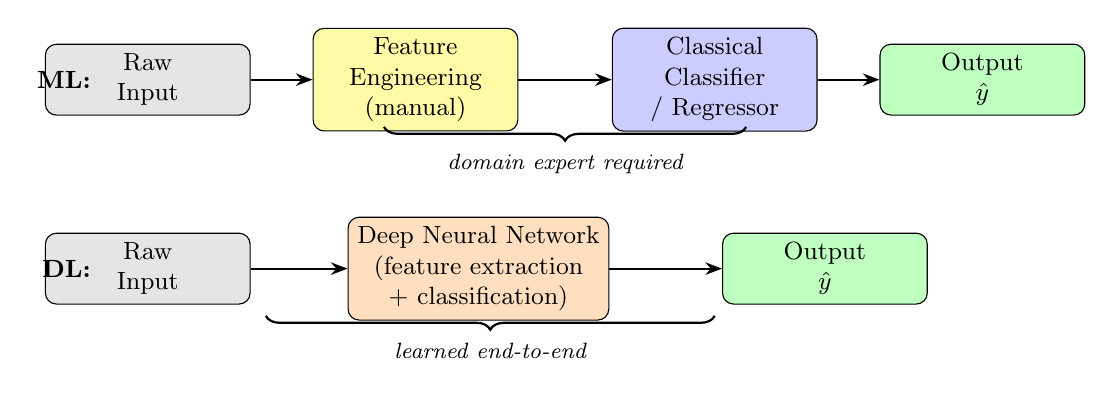
\begin{tikzpicture}[
    box/.style={draw, rounded corners, fill=#1, minimum width=2.6cm,
                minimum height=0.9cm, align=center, font=\small},
    arr/.style={-{Stealth[length=6pt]}, thick},
    every node/.style={font=\small}
  ]

  %% ---- Classical Machine Learning row ----
  \node[box=gray!20]  (input_ml)  at (0,0)      {Raw\\Input};
  \node[box=yellow!35](feat_ml)   at (3.4,0)    {Feature\\Engineering\\(manual)};
  \node[box=blue!20]  (model_ml)  at (7.2,0)    {Classical\\Classifier\\/ Regressor};
  \node[box=green!25] (out_ml)    at (10.6,0)   {Output\\$\hat{y}$};

  \draw[arr] (input_ml)  -- (feat_ml);
  \draw[arr] (feat_ml)   -- (model_ml);
  \draw[arr] (model_ml)  -- (out_ml);

  \node[font=\small\bfseries, anchor=east] at (-0.6,0) {ML:};

  %% ---- Deep Learning row ----
  \node[box=gray!20]  (input_dl)  at (0,-2.4)  {Raw\\Input};
  \node[box=orange!25](dl_block)  at (4.2,-2.4){Deep Neural Network\\(feature extraction\\+ classification)};
  \node[box=green!25] (out_dl)    at (8.6,-2.4){Output\\$\hat{y}$};

  \draw[arr] (input_dl)  -- (dl_block);
  \draw[arr] (dl_block)  -- (out_dl);

  \node[font=\small\bfseries, anchor=east] at (-0.6,-2.4) {DL:};

  %% ---- annotation braces ----
  \draw[decorate,decoration={brace,mirror,amplitude=5pt},thick]
    (3.0,-0.6) -- (7.6,-0.6)
    node[midway, below=6pt, font=\footnotesize\itshape]
      {domain expert required};

  \draw[decorate,decoration={brace,mirror,amplitude=5pt},thick]
    (1.5,-3.0) -- (7.2,-3.0)
    node[midway, below=6pt, font=\footnotesize\itshape]
      {learned end-to-end};

\end{tikzpicture}
\caption{Classical ML vs.\ Deep Learning pipelines (Slide V09).
In classical ML the feature engineering block is separate and requires
domain expertise; in deep learning it is subsumed within the network and
learned automatically from data.}
\label{fig:ml_vs_dl}
\end{figure}

\subsection{A Simple Feedforward Neural Network}
\label{subsec:ffnn_diagram}

\cref{fig:ffnn} illustrates a two-hidden-layer feedforward network, the type
built in the Week~1 hands-on session.

\begin{figure}[ht]
\centering
\begin{tikzpicture}[
    neuron/.style={circle, draw, fill=#1, minimum size=0.75cm, inner sep=0pt},
    arr/.style={-{Stealth[length=5pt]}, gray!70},
    lbl/.style={font=\scriptsize\bfseries, align=center}
  ]

  \def\layersep{2.6cm}

  %% Input layer (4 nodes)
  \foreach \y/\name in {1.5/x_1, 0.5/x_2, -0.5/x_3, -1.5/x_4}{
    \node[neuron=cyan!25] (I\name) at (0,\y) {};
    \node[font=\tiny] at (0,\y) {$\name$};
  }

  %% Hidden layer 1 (5 nodes)
  \foreach \y in {2, 1, 0, -1, -2}{
    \node[neuron=yellow!35] (H1-\y) at (\layersep,\y) {};
  }

  %% Hidden layer 2 (4 nodes)
  \foreach \y in {1.5, 0.5, -0.5, -1.5}{
    \node[neuron=orange!35] (H2-\y) at (2*\layersep,\y) {};
  }

  %% Output layer (3 nodes)
  \foreach \y/\name in {1/y_1, 0/y_2, -1/y_3}{
    \node[neuron=green!35] (O\name) at (3*\layersep,\y) {};
    \node[font=\tiny] at (3*\layersep,\y) {$\name$};
  }

  %% Connections: input -> H1
  \foreach \src in {x_1,x_2,x_3,x_4}{
    \foreach \dst in {2,1,0,-1,-2}{
      \draw[arr] (I\src) -- (H1-\dst);
    }
  }

  %% Connections: H1 -> H2
  \foreach \src in {2,1,0,-1,-2}{
    \foreach \dst in {1.5,0.5,-0.5,-1.5}{
      \draw[arr] (H1-\src) -- (H2-\dst);
    }
  }

  %% Connections: H2 -> output
  \foreach \src in {1.5,0.5,-0.5,-1.5}{
    \foreach \dst in {y_1,y_2,y_3}{
      \draw[arr] (H2-\src) -- (O\dst);
    }
  }

  %% Layer labels
  \node[lbl] at (0,-2.8)         {Input\\Layer};
  \node[lbl] at (\layersep,-2.8) {Hidden\\Layer 1};
  \node[lbl] at (2*\layersep,-2.8){Hidden\\Layer 2};
  \node[lbl] at (3*\layersep,-2.8){Output\\Layer};

\end{tikzpicture}
\caption{A fully-connected feedforward neural network with two hidden layers
(4-5-4-3 architecture).  This is the architecture built in the Week~1
hands-on session.  Each arrow represents a learnable weight $w_{jk}$.}
\label{fig:ffnn}
\end{figure}

%% ============================================================
\section{Key Concepts: Backpropagation and Gradient Descent}
\label{sec:backprop}
%% ============================================================

\subsection{Gradient Descent}
\label{subsec:gd}

The standard parameter update rule is stochastic gradient descent (SGD):
\begin{equation}
  \label{eq:sgd}
  \boldsymbol{\theta}^{(t+1)}
  = \boldsymbol{\theta}^{(t)}
  - \eta \, \nabla_{\boldsymbol{\theta}} \mathcal{L}\!\left(\boldsymbol{\theta}^{(t)}\right),
\end{equation}
where $\eta > 0$ is the learning rate and $\nabla_{\boldsymbol{\theta}}
\mathcal{L}$ is the gradient of the loss with respect to the parameters.

\subsection{The Backpropagation Algorithm}
\label{subsec:bp_algo}

Backpropagation efficiently computes $\nabla_{\boldsymbol{\theta}} \mathcal{L}$
by a single forward pass (to cache activations) followed by a single backward
pass (to propagate error signals).

\begin{algorithm}[H]
\caption{Backpropagation for a fully-connected network}
\label{alg:backprop}
\SetAlgoLined
\KwIn{Training pair $(\mathbf{x}, y)$; weights $\{(\mathbf{W}^{(l)}, \mathbf{b}^{(l)})\}_{l=1}^{L+1}$;
      learning rate $\eta$; activation $\phi$}
\KwOut{Updated weights}

\BlankLine
\tcp{--- Forward Pass ---}
$\mathbf{a}^{(0)} \leftarrow \mathbf{x}$\;
\For{$l = 1$ \KwTo $L+1$}{
  $\mathbf{z}^{(l)} \leftarrow \mathbf{W}^{(l)}\mathbf{a}^{(l-1)} + \mathbf{b}^{(l)}$\;
  $\mathbf{a}^{(l)} \leftarrow \phi(\mathbf{z}^{(l)})$ \tcp*{element-wise}
}
Compute loss $\mathcal{L} = \ell(y, \mathbf{a}^{(L+1)})$\;

\BlankLine
\tcp{--- Backward Pass ---}
$\boldsymbol{\delta}^{(L+1)} \leftarrow \nabla_{\mathbf{a}^{(L+1)}}\mathcal{L}
                                \odot \phi'(\mathbf{z}^{(L+1)})$\;
\For{$l = L$ \KwTo $1$}{
  $\boldsymbol{\delta}^{(l)} \leftarrow
    \left(\mathbf{W}^{(l+1)\top}\boldsymbol{\delta}^{(l+1)}\right)
    \odot \phi'(\mathbf{z}^{(l)})$\;
}

\BlankLine
\tcp{--- Weight Update ---}
\For{$l = 1$ \KwTo $L+1$}{
  $\mathbf{W}^{(l)} \leftarrow \mathbf{W}^{(l)}
    - \eta\, \boldsymbol{\delta}^{(l)} {\mathbf{a}^{(l-1)}}^{\!\top}$\;
  $\mathbf{b}^{(l)} \leftarrow \mathbf{b}^{(l)}
    - \eta\, \boldsymbol{\delta}^{(l)}$\;
}
\Return Updated weights\;
\end{algorithm}

\begin{keyinsight}[title=Why BP Fails in Deep Networks]
In \cref{alg:backprop}, the backward-pass loop multiplies error signals
by $\mathbf{W}^{(l)\top}$ at each layer.  If the spectral norm
$\|\mathbf{W}^{(l)}\|_2 < 1$ (common with random initialisation) or
$|\phi'(z)| \ll 1$ (sigmoid saturation), the signals in early layers
vanish exponentially with depth.  This is the \emph{vanishing gradient
problem} that blocked progress until the 2006 Hinton breakthrough and the
subsequent adoption of ReLU activations ($\phi(z) = \max(0,z)$, derivative
$= 1$ for $z>0$).
\end{keyinsight}

\subsection{Greedy Layer-Wise Pre-Training}
\label{subsec:greedy}

The algorithmic insight of Hinton \emph{et al.}\ (2006) is to decompose the
deep training problem into a sequence of shallow problems:

\begin{enumerate}
  \item Train Layer~1 as an RBM on the raw data $\{\mathbf{x}_i\}$.
  \item Use the hidden representations from Layer~1 as inputs to train
        Layer~2 as a second RBM.
  \item Continue greedily for all $L$ layers.
  \item Use the stacked pre-trained weights to initialise the full deep
        network, then fine-tune end-to-end with BP.
\end{enumerate}

The energy function of an RBM is:
\begin{equation}
  \label{eq:rbm_energy}
  E(\mathbf{v}, \mathbf{h}) = -\mathbf{b}^\top \mathbf{v}
                              - \mathbf{c}^\top \mathbf{h}
                              - \mathbf{v}^\top \mathbf{W} \mathbf{h},
\end{equation}
where $\mathbf{v}$ are visible units, $\mathbf{h}$ are hidden units,
$\mathbf{b}$, $\mathbf{c}$ are biases, and $\mathbf{W}$ are the RBM weights.
The joint distribution is:
\begin{equation}
  \label{eq:rbm_joint}
  P(\mathbf{v},\mathbf{h}) = \frac{1}{Z}\exp\!\left(-E(\mathbf{v},\mathbf{h})\right),
  \qquad Z = \sum_{\mathbf{v},\mathbf{h}} \exp\!\left(-E(\mathbf{v},\mathbf{h})\right).
\end{equation}

%% ============================================================
\section{Why Sequence Models? Motivating Example}
\label{sec:seqmodels}
%% ============================================================

Standard feedforward networks and CNNs process inputs as fixed-size
\emph{static} feature vectors; they cannot model the order in which elements
appear.  The instructor motivates sequence models with a concrete example:

\begin{example}[title=Mobile Phone Number Recognition]
All Indian mobile numbers are 10-digit strings drawn from the alphabet
$\{0,1,\ldots,9\}$.  Two different numbers, say $9876543210$ and $9801234567$,
use exactly the same digit set.  Their \emph{distribution} of digits
is similar, but their \emph{sequential ordering} is completely different.

A feedforward classifier operating on a bag-of-digits feature (histogram of
digit occurrences) would be unable to distinguish the two numbers.  Only a
model that respects the temporal order — a Recurrent Neural Network —
can capture this discriminatory information.
\end{example}

\begin{keyinsight}
This motivating example generalises widely: speech (phoneme sequences),
text (word sequences), DNA (nucleotide sequences), financial time-series
(price sequences) — in all of these, the \emph{order matters}.
Recurrent Neural Networks (RNNs), LSTMs, GRUs, and Transformers were all
developed to exploit this sequential structure.
\end{keyinsight}

Formally, a vanilla RNN processes a sequence $x_1, x_2, \ldots, x_T$ by
maintaining a hidden state $\mathbf{h}_t$:
\begin{align}
  \label{eq:rnn}
  \mathbf{h}_t &= \phi\!\left(\mathbf{W}_h\, \mathbf{h}_{t-1}
                              + \mathbf{W}_x\, \mathbf{x}_t
                              + \mathbf{b}\right), \\
  \mathbf{o}_t &= \mathbf{V}\, \mathbf{h}_t,
\end{align}
where $\mathbf{W}_h$, $\mathbf{W}_x$, $\mathbf{V}$, $\mathbf{b}$ are shared
parameters across all time steps $t$.

%% ============================================================
\section{Summary and Looking Ahead}
\label{sec:summary}
%% ============================================================

\subsection{Session Summary}
\label{subsec:session_summary}

Session~01 served as a complete orientation to the Deep Learning course.
The key take-home messages are:

\begin{enumerate}[label=\textbf{T\arabic*.}]
  \item \textbf{Course design}: The course is hands-on and PyTorch-driven,
        spanning perceptrons (Week~1) through Transformers and Generative
        Models (Weeks~8--13).
  \item \textbf{The 2006 breakthrough}: Geoffrey Hinton \emph{et al.}\ showed
        for the first time that a deep neural network could be reliably trained
        and that doing so yields state-of-the-art performance.  This paper
        re-ignited the field and is the root of modern AI.
  \item \textbf{Classical ML vs.\ Deep Learning}: Classical ML uses manual
        feature engineering followed by a shallow model; Deep Learning learns
        features and classification jointly, end-to-end, from raw data.
  \item \textbf{The AI hierarchy}: AI $\supset$ ML $\supset$ NN $\supset$ DL
        $\supset$ GAI.  This course focuses on NN, DL, and GAI.
  \item \textbf{Three pillars of success}: algorithmic advances
        (pre-training, ReLU, normalisation), big data, and GPU computing.
  \item \textbf{Sequence models}: RNNs and their variants (LSTM, GRU,
        Transformer) are necessary when discriminatory information lies in
        the \emph{order} of inputs, not just their distribution.
\end{enumerate}

\subsection{What the Student Should Know After This Course}
\label{subsec:takeaway}

Quoting the instructor verbatim:
\begin{quote}
``If you have done the deep learning course, you should be very comfortable
with Convolutional Networks.  You should be very comfortable with LSTM.
You should have very good working experience with Transformers and Generative
Adversarial Networks.  That should be the take-home message for all of you
when you have gone through this course.''
--- Prof.\ S R M Prasanna
\end{quote}

\subsection{Connections to Upcoming Sessions}
\label{subsec:upcoming}

\begin{table}[ht]
\centering
\caption{Road map from Session~01 to the rest of the course.}
\label{tab:roadmap}
\begin{tabular}{lll}
\toprule
\textbf{Phase} & \textbf{Sessions} & \textbf{Core Concept Introduced} \\
\midrule
Foundations    & 1--2  & Perceptron, BP, 2-layer NN \\
Deep NNs       & 3--4  & Deep MLP, vanishing gradients, pre-training \\
Spatial models & 5--8  & Convolutional networks, pooling, Grad-CAM \\
Sequence models& 9--12 & RNN, BPTT, LSTM, GRU \\
Attention      & 13--14 & Seq2Seq, Bahdanau attention, Transformer \\
Generative     & 15--18 & VAE, GAN, GPT \\
\bottomrule
\end{tabular}
\end{table}

\begin{keyinsight}[title=The Big Picture]
The entire curriculum can be understood through one lens: each successive
architecture relaxes a bottleneck of its predecessor.
\begin{itemize}
  \item Perceptron $\to$ MLP: adds non-linearity and hidden representations.
  \item MLP $\to$ Deep MLP: adds depth for hierarchical abstraction.
  \item Deep MLP $\to$ CNN: adds spatial inductive bias (weight sharing,
        local connectivity).
  \item CNN/MLP $\to$ RNN: adds temporal inductive bias (recurrence).
  \item RNN $\to$ LSTM: adds gating to solve the long-range dependency problem.
  \item RNN $\to$ Transformer: replaces recurrence with self-attention for
        parallelisable, global-context modelling.
  \item Transformer $\to$ GAI models: repurposes the Transformer as a
        conditional generative model.
\end{itemize}
\end{keyinsight}

\newpage
%% ============================================================
%%  Appendix
%% ============================================================
\appendix

\section{Activation Functions Reference}
\label{app:activations}

\begin{table}[ht]
\centering
\caption{Common activation functions used in deep networks.}
\label{tab:activations}
\begin{tabular}{llll}
\toprule
\textbf{Name} & \textbf{Formula} $\phi(z)$ & \textbf{Derivative} $\phi'(z)$ & \textbf{Range} \\
\midrule
Sigmoid   & $\dfrac{1}{1+e^{-z}}$          & $\phi(z)(1-\phi(z))$          & $(0,1)$ \\[8pt]
Tanh      & $\dfrac{e^z - e^{-z}}{e^z+e^{-z}}$ & $1-\phi(z)^2$            & $(-1,1)$ \\[8pt]
ReLU      & $\max(0,z)$                     & $\mathbf{1}[z>0]$             & $[0,\infty)$ \\[8pt]
Leaky ReLU & $\max(\alpha z,z)$, $\alpha\ll 1$ & $1$ if $z>0$, else $\alpha$ & $(-\infty,\infty)$ \\[8pt]
Softmax   & $\dfrac{e^{z_k}}{\sum_j e^{z_j}}$ & (Jacobian matrix)          & $(0,1)$ \\
\bottomrule
\end{tabular}
\end{table}

\begin{remark}
\label{rem:relu}
The switch from sigmoid/tanh to ReLU activations was one of the most
impactful practical innovations of the 2010s.  Because $\phi'(z)=1$ for
$z>0$, ReLU does not suppress gradients in the backward pass, substantially
mitigating the vanishing gradient problem (see \cref{eq:vanishing}).
\end{remark}

\section{Glossary}
\label{app:glossary}

\begin{description}[style=nextline]
  \item[Artificial Intelligence (AI)]
    The broad field of creating computing systems that mimic human
    intelligence.

  \item[Machine Learning (ML)]
    A subfield of AI where systems learn from data without being explicitly
    programmed.

  \item[Neural Network (NN)]
    A layered computational graph of artificial neurons; the precursor to
    deep learning.

  \item[Deep Learning (DL)]
    ML with multi-layer neural networks that learn hierarchical
    representations from raw data.

  \item[Generative AI (GAI)]
    Deep learning models that generate new data samples (text, images,
    audio) from a learned distribution.

  \item[Backpropagation (BP)]
    Algorithm for computing gradients of the loss through a neural network
    using the chain rule of calculus.

  \item[Vanishing Gradient]
    The exponential decay of gradient signals in early layers of a deep
    network, caused by repeated multiplication by small derivative values.

  \item[Greedy Layer-wise Pre-training]
    A technique introduced by Hinton \emph{et al.}\ (2006) for training deep
    networks by successively training each layer as an RBM before global
    fine-tuning.

  \item[Restricted Boltzmann Machine (RBM)]
    A two-layer energy-based generative model used as the building block
    of Deep Belief Networks.

  \item[Convolutional Neural Network (CNN)]
    A deep network with weight-shared, locally-connected filters designed
    for spatially-structured inputs (images).

  \item[Recurrent Neural Network (RNN)]
    A network with cyclic connections that maintains a hidden state over
    time steps, enabling sequence modelling.

  \item[Long Short-Term Memory (LSTM)]
    An RNN variant with multiplicative gating mechanisms that mitigate
    the vanishing gradient problem in long sequences.

  \item[Transformer]
    An architecture based entirely on self-attention (no recurrence) that
    models global dependencies in sequences.  Foundation of GPT and BERT.

  \item[Variational Autoencoder (VAE)]
    A generative model that learns a latent-space distribution and can
    sample new data by decoding latent vectors.

  \item[Generative Adversarial Network (GAN)]
    A generative model consisting of a Generator and a Discriminator
    trained adversarially.

  \item[PyTorch]
    An open-source deep learning framework developed by Meta AI.  Used
    throughout this course for hands-on implementations.
\end{description}

\clearpage

%% ============================================================
%% Session 02: Tensors in PyTorch
%% ============================================================
\part{Session 02: Tensors in PyTorch}

% ==================================================================

% ------------------------------------------------------------------
% Title page
% ------------------------------------------------------------------
\begin{titlepage}
  \centering
  \vspace*{2cm}
  {\LARGE\bfseries Deep Learning Course\\[0.4em]
   \large Indian Institute of Information Technology Dharwad\par}
  \vspace{1.5cm}
  \rule{\linewidth}{0.5pt}\\[0.6em]
  {\Huge\bfseries Session 02\\[0.3em]
   \LARGE Tensors in PyTorch\par}
  \rule{\linewidth}{0.5pt}\\[1.2cm]

  \begin{tabular}{rl}
    \tbf{Instructors:}  & Prof.\ S R M Prasanna \& Dr.\ Sunil Saumya \\[4pt]
    \tbf{Department:}   & Data Science \& Artificial Intelligence \\[4pt]
    \tbf{Institute:}    & IIIT Dharwad \\[4pt]
    \tbf{Date:}         & November 20, 2025 \\[4pt]
    \tbf{Slide Deck:}   & \texttt{02-PyTorchDL-Tensor} (17 slides) \\[4pt]
    \tbf{Notebook:}     & \texttt{TensorBasics.ipynb} \\[4pt]
    \tbf{Duration:}     & 1 hour 44 minutes \\[4pt]
    \tbf{Video:}        & \url{https://vimeo.com/1139558263} \\
  \end{tabular}

  \vfill
  {\large\itshape ``Tensors are the fundamental data structure of deep learning.
   Master them and you master the language of neural networks.''\par}
  \vspace{1cm}
\end{titlepage}

% ------------------------------------------------------------------
% Table of contents
% ------------------------------------------------------------------

\newpage

% ==================================================================
\section{Introduction}
\label{sec:intro}
% ==================================================================

Session~02 of the Deep Learning course at IIIT Dharwad is a hands-on
laboratory session dedicated to \tbf{PyTorch tensors}. The session is
structured as a live Google Colab coding walkthrough using the notebook
\ttt{TensorBasics.ipynb}, supported by the 17-slide deck
\ttt{02-PyTorchDL-Tensor}.

The instructors began with a brief recap of Session~01, which covered the
course plan, a high-level overview of machine learning and deep learning, and
the reasons for choosing PyTorch over TensorFlow. The key motivation for this
session is captured in the course philosophy:

\begin{quote}
  \itshape ``This course will be 50\% theory (mathematics and conceptual
  understanding) and 50\% practice (coding), because that is what will help you
  immediately in your projects and workplace.''
  \upshape \quad --- Dr.\ Sunil Saumya (00:11:55)
\end{quote}

The session covers the following major topics in sequence:
\begin{enumerate}[label=\arabic*.]
  \item Why tensors? GPU support, autograd, and the computation graph.
  \item Tensor dimensions: scalars, vectors, matrices, and higher-order tensors.
  \item Tensor creation functions: \ttt{torch.tensor}, \ttt{torch.zeros},
        \ttt{torch.ones}, \ttt{torch.randn}, \ttt{torch.arange},
        \ttt{torch.linspace}, \ttt{torch.eye}, \ttt{torch.full}.
  \item Tensor shapes and data types (\ttt{dtype}).
  \item Mathematical operations: unary, element-wise, reduction.
  \item Matrix multiplication and the neural network forward pass
        $\mathbf{Y} = \mathbf{W}\mathbf{X} + \mathbf{B}$.
\end{enumerate}

% ==================================================================
\section{Background and Prerequisites}
\label{sec:background}
% ==================================================================

\subsection{What is a Tensor?}

\begin{definition}[Tensor]
\label{def:tensor}
A \tbf{tensor} is a multi-dimensional array of numerical values. It generalises
the notions of scalars (0-D), vectors (1-D), and matrices (2-D) to an arbitrary
number of dimensions. In the context of PyTorch, tensors additionally support
GPU-accelerated computation and automatic differentiation.
\end{definition}

Tensors are structurally similar to NumPy \ttt{ndarray} objects but differ in
two critical respects:

\begin{itemize}[leftmargin=*]
  \item \tbf{GPU compatibility.} Tensors can be allocated on CUDA-enabled
        GPUs, enabling massive parallelism. The CUDA check in the notebook
        confirmed \texttt{torch.cuda.is\_available() = True} with PyTorch
        version \ttt{2.9.0+cu126}.
  \item \tbf{Automatic differentiation (autograd).} PyTorch tracks operations
        on tensors in a dynamic computation graph, enabling automatic
        gradient computation via backpropagation.
\end{itemize}

\subsection{Tensor Dimensions}

\Cref{tab:tensor-dims} summarises the tensor hierarchy by dimensionality and
provides deep learning examples for each rank.

\begin{table}[ht]
  \centering
  \caption{Tensor ranks, shapes, and deep learning use cases.}
  \label{tab:tensor-dims}
  \begin{tabularx}{\linewidth}{c c X X}
    \toprule
    \tbf{Rank} & \tbf{Name} & \tbf{Shape example} & \tbf{Deep Learning use case} \\
    \midrule
    0 & Scalar     & \ttt{()} or \ttt{[]}    & Loss value, learning rate, single metric \\
    1 & Vector     & \ttt{[n]}               & Bias vector, 1-D feature vector \\
    2 & Matrix     & \ttt{[m, n]}            & Weight matrix, batch of vectors \\
    3 & 3-D Tensor & \ttt{[batch, seq, feat]}& Sequence data (NLP), time series \\
    4 & 4-D Tensor & \ttt{[B, C, H, W]}      & Image batches (CNNs) \\
    5 & 5-D Tensor & \ttt{[B, D, C, H, W]}   & Video data (3-D CNNs) \\
    \bottomrule
  \end{tabularx}
\end{table}

\begin{keyinsight}[title=Tensors vs.\ NumPy Arrays]
Up to 3 dimensions, tensors and NumPy arrays are visually and structurally
identical. The difference becomes apparent at dimensions 4 and above, where
tensors provide a natural and efficient representation for data such as
image batches (\ttt{[B, C, H, W]}) that would be unwieldy to reason about
in plain NumPy.
\end{keyinsight}

\subsection{PyTorch vs.\ TensorFlow}

Both PyTorch and TensorFlow use tensors as their primary data structure, but
PyTorch's dynamic computation graph (define-by-run) makes it the framework
of choice for research and this course. TensorFlow uses a static graph
(define-then-run) by default in its original design, though TensorFlow 2.x
introduced eager execution. The course uses PyTorch exclusively.

% ==================================================================
\section{Tensor Creation in PyTorch}
\label{sec:creation}
% ==================================================================

\subsection{Environment Setup}

The session opened with a GPU availability check. This should always be the
first step in a PyTorch Colab notebook to confirm that training-speed hardware
is accessible.

\begin{lstlisting}[caption={Environment setup and GPU check (V03, 00:16:00).},
                   label={lst:setup}]
import torch
print(torch.__version__)     # Output: 2.9.0+cu126

if torch.cuda.is_available():
    print("cuda is available")
else:
    print("cuda is not available")
# Output: cuda is available
\end{lstlisting}

\subsection{Primary Creation Functions}

PyTorch provides two broad classes of creation functions:
(1) \tbf{data-initialised} tensors, created from existing Python data, and
(2) \tbf{factory functions}, which generate tensors of a specified shape
filled according to some rule (zeros, ones, random, etc.).

\subsubsection{Data-Initialised Tensors}

\begin{lstlisting}[caption={Creating tensors from data (V04, 00:21:50).},
                   label={lst:from-data}]
# From a Python nested list -- preserves dtype
a = torch.tensor([[1, 2, 3],
                  [4, 5, 6]])
# tensor([[1, 2, 3],
#         [4, 5, 6]])

# Uninitialized -- raw memory, values are garbage
b = torch.empty(2, 3)
# tensor([[1.5163e-19,  6.8316e+22,  7.1235e+28],
#         [4.6116e-24,  1.2323e+25,  7.7783e+31]])
\end{lstlisting}

\begin{warningbox}
\ttt{torch.empty()} allocates raw memory \tbf{without initialisation}.
The values returned are whatever bytes happened to be in that memory
location --- they are not zero. Only use \ttt{torch.empty} when you
plan to immediately overwrite the tensor contents.
\end{warningbox}

\subsubsection{Factory Functions: Zeros, Ones, and Random}

\begin{lstlisting}[caption={Factory functions (V05, 00:25:24).},
                   label={lst:factory}]
# All zeros
torch.zeros(2, 3)
# tensor([[0., 0., 0.],
#         [0., 0., 0.]])

# All ones
e = torch.ones(2, 3)
# tensor([[1., 1., 1.],
#         [1., 1., 1.]])

# Random normal: mean=0, std=1
e = torch.randn(2, 3)
# tensor([[ 0.0856,  0.2067,  0.6007],
#         [ 0.4394,  0.7040,  0.9578]])
\end{lstlisting}

\begin{keyinsight}[title=Weight Initialisation with \ttt{torch.randn}]
Neural network weights are almost always initialised from a random normal
distribution $\mathcal{N}(0, 1)$ using \ttt{torch.randn()}. Proper
initialisation is critical: weights that are too large cause exploding
gradients; weights that are too small cause vanishing gradients.
\end{keyinsight}

\subsubsection{Reproducibility: \ttt{torch.manual\_seed}}

\begin{lstlisting}[caption={Random seed for reproducibility (V06, 00:30:04).},
                   label={lst:seed}]
# Without seed -- different values on every run
e = torch.randn(2, 3)
# tensor([[ 0.2793,  0.2515, -0.0420],
#         [-0.3960,  0.3256,  0.9385]])

# With seed -- identical values every run
torch.manual_seed(10)
e = torch.randn(2, 3)
# tensor([[ 0.3374,  0.6029,  0.3133],
#         [-0.4156,  0.3219,  0.4119]])
\end{lstlisting}

\begin{keyinsight}[title=Why Seeds Matter]
Setting \ttt{torch.manual\_seed(n)} before any random operation ensures
that the pseudo-random number generator (PRNG) starts from the same state,
producing the same sequence of values on every run. This is essential for
\tbf{reproducible experiments}: two researchers running the same notebook
with the same seed will obtain identical results, making debugging and
scientific comparison reliable.
\end{keyinsight}

\subsubsection{Sequential and Structured Tensors}

\begin{lstlisting}[caption={\ttt{arange}, \ttt{linspace}, \ttt{eye}, \ttt{full}
                   (V07--V08, 00:33:05--00:35:05).},
                   label={lst:structured}]
# torch.arange -- like Python range(), creates integer sequence
torch.arange(0, 10)
# tensor([0, 1, 2, 3, 4, 5, 6, 7, 8, 9])

# torch.linspace -- N evenly spaced points between a and b
torch.linspace(0, 1, 5)
# tensor([0.0000, 0.2500, 0.5000, 0.7500, 1.0000])

# torch.eye -- identity matrix
torch.eye(3)
# tensor([[1., 0., 0.],
#         [0., 1., 0.],
#         [0., 0., 1.]])

# torch.full -- fill with constant value
torch.full((2, 3), 10)
# tensor([[10., 10., 10.],
#         [10., 10., 10.]])
\end{lstlisting}

\begin{example}[title=\ttt{arange} vs.\ \ttt{linspace}]
\begin{itemize}[leftmargin=*]
  \item \ttt{torch.arange(start, stop, step)} takes a \tbf{step size}. The
        exact number of output elements depends on the range and step.
  \item \ttt{torch.linspace(start, stop, n)} takes a \tbf{count}. You always
        get exactly $n$ evenly spaced values from \ttt{start} to \ttt{stop}
        (inclusive).
\end{itemize}
Use \ttt{linspace} when you need a precise number of sample points, e.g.\
when creating a grid for function plotting or interpolation.
\end{example}

% ------------------------------------------------------------------
% TikZ diagram 1: Tensor creation function tree
% ------------------------------------------------------------------
\subsection{Creation Function Overview}

\Cref{fig:creation-tree} provides a visual overview of the PyTorch tensor
creation functions covered in this session.

\begin{figure}[ht]
  \centering
  \begin{tikzpicture}[
      node distance=1.2cm and 2.2cm,
      every node/.style={font=\small},
      box/.style={rectangle, rounded corners=3pt, draw=codeblue,
                  fill=blue!8, minimum width=2.8cm, minimum height=0.7cm,
                  align=center},
      root/.style={rectangle, rounded corners=4pt, draw=codeblue!80!black,
                   fill=codeblue!20, minimum width=3.4cm, minimum height=0.8cm,
                   align=center, font=\small\bfseries},
      catbox/.style={rectangle, rounded corners=3pt, draw=gray!70,
                     fill=gray!12, minimum width=3cm, minimum height=0.7cm,
                     align=center, font=\small\itshape},
      arr/.style={-{Stealth[length=5pt]}, gray!70, thick},
    ]
    % Root
    \node[root] (root) {Tensor Creation};

    % Category nodes
    \node[catbox, below left=1.2cm and 3.5cm of root]  (fromdata) {From Data};
    \node[catbox, below=1.2cm of root]                  (factory)  {Factory};
    \node[catbox, below right=1.2cm and 3.5cm of root] (structured){Structured};

    % From-data children
    \node[box, below=0.8cm of fromdata] (tensor) {\ttt{torch.tensor()}};
    \node[box, below=0.4cm of tensor]   (empty)  {\ttt{torch.empty()}};

    % Factory children
    \node[box, below left=0.8cm and 0.8cm of factory]  (zeros) {\ttt{torch.zeros()}};
    \node[box, below=0.8cm of factory]                  (ones)  {\ttt{torch.ones()}};
    \node[box, below right=0.8cm and 0.8cm of factory] (randn) {\ttt{torch.randn()}};

    % Structured children
    \node[box, below left=0.8cm and 0.6cm of structured]  (arange)   {\ttt{torch.arange()}};
    \node[box, below=0.8cm of structured]                  (linspace) {\ttt{torch.linspace()}};
    \node[box, below right=0.8cm and 0.6cm of structured] (eye)      {\ttt{torch.eye()}};
    \node[box, below=2.0cm of eye]                         (full)     {\ttt{torch.full()}};

    % Arrows root -> categories
    \draw[arr] (root.south) -- (fromdata.north);
    \draw[arr] (root.south) -- (factory.north);
    \draw[arr] (root.south) -- (structured.north);

    % Arrows fromdata
    \draw[arr] (fromdata.south) -- (tensor.north);
    \draw[arr] (fromdata.south) -- (empty.north);

    % Arrows factory
    \draw[arr] (factory.south) -- (zeros.north);
    \draw[arr] (factory.south) -- (ones.north);
    \draw[arr] (factory.south) -- (randn.north);

    % Arrows structured
    \draw[arr] (structured.south) -- (arange.north);
    \draw[arr] (structured.south) -- (linspace.north);
    \draw[arr] (structured.south) -- (eye.north);
    \draw[arr] (structured.south) -- (full.north);
  \end{tikzpicture}
  \caption{PyTorch tensor creation functions covered in Session~02,
           organised by category.}
  \label{fig:creation-tree}
\end{figure}

% ==================================================================
\section{Tensor Shapes and Data Types}
\label{sec:shapes-dtypes}
% ==================================================================

\subsection{Shape Manipulation}
\label{subsec:shapes}

Every tensor has a \tbf{shape} attribute (\ttt{x.shape}) that returns a
\ttt{torch.Size} object --- essentially a tuple of dimension sizes.

\begin{lstlisting}[caption={Shape inspection and reshape (V09, 00:37:35).},
                   label={lst:shapes}]
x = torch.tensor([[1, 2, 3],
                  [4, 5, 6]])      # shape: (2, 3)
print(x.shape)                    # torch.Size([2, 3])

# Reshape: same data, different view
x.reshape(3, 2)
# tensor([[1, 2],
#         [3, 4],
#         [5, 6]])

# 3D tensor
torch.full((2, 3, 10), 10).shape  # torch.Size([2, 3, 10])
\end{lstlisting}

\begin{remark}
\label{rem:reshape}
\ttt{reshape} does not copy data when the new shape is compatible with the
memory layout of the original tensor; it returns a \tbf{view}. When a copy
is required (e.g.\ for non-contiguous tensors), use \ttt{.contiguous()}
followed by \ttt{.reshape()}, or use \ttt{.view()}.
\end{remark}

\subsection{Data Types (\ttt{dtype})}
\label{subsec:dtypes}

Each PyTorch tensor has a fixed numerical precision encoded in its \ttt{dtype}
attribute. \Cref{tab:dtypes} summarises the most commonly used types.

\begin{table}[ht]
  \centering
  \caption{Common PyTorch \ttt{dtype} values and their deep learning roles.}
  \label{tab:dtypes}
  \begin{tabular}{llll}
    \toprule
    \tbf{\ttt{dtype}} & \tbf{Bits} & \tbf{Range / Precision} & \tbf{Use Case} \\
    \midrule
    \ttt{torch.int64}   & 64 & Integer, large range    & Indices, integer ops \\
    \ttt{torch.float32} & 32 & $\sim$7 decimal digits  & Standard NN weights \& activations \\
    \ttt{torch.float64} & 64 & $\sim$15 decimal digits & High-precision (slower on GPU) \\
    \ttt{torch.float16} & 16 & $\sim$3 decimal digits  & Quantisation, memory reduction \\
    \ttt{torch.int8}    &  8 & $-128$ to $127$         & Extreme quantisation (LLM inference) \\
    \bottomrule
  \end{tabular}
\end{table}

\begin{lstlisting}[caption={dtype inspection and type casting (V10, 00:39:49).},
                   label={lst:dtype}]
x = torch.tensor([[1, 2, 3], [4, 5, 6]])
x.dtype     # torch.int64  (integers inferred)

y = torch.tensor([[1.0, 2.0, 3.0], [5.0, 6.0, 7.0]])
y.dtype     # torch.float32 (floats inferred)

# Explicit type casting
x.float()   # converts to torch.float32
x.double()  # converts to torch.float64
x.half()    # converts to torch.float16
\end{lstlisting}

\begin{keyinsight}[title=Quantisation and Large Language Models]
Large language models (LLMs) typically use \ttt{float16} (\ttt{fp16}) or
even \ttt{int8} precision to reduce GPU memory footprint during inference.
A model that requires 32~GB in \ttt{float32} requires only 16~GB in
\ttt{float16} and 8~GB in \ttt{int8}. This precision--efficiency trade-off
is a central technique in deploying modern deep learning systems.
\end{keyinsight}

% ------------------------------------------------------------------
% TikZ diagram 2: dtype precision ladder
% ------------------------------------------------------------------
\begin{figure}[ht]
  \centering
  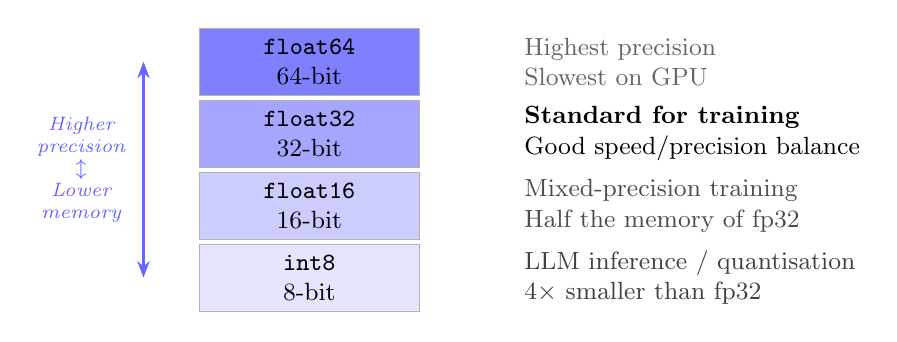
\begin{tikzpicture}[
      node distance=0.0cm,
      every node/.style={font=\small},
      dblock/.style={rectangle, draw=gray!60, fill=blue!#1, minimum width=2.8cm,
                     minimum height=0.85cm, align=center},
    ]
    % Stack of dtype blocks (left column: label; right column: bits)
    \node[dblock=50] (fp64) at (0,0)     {\ttt{float64} \\ 64-bit};
    \node[dblock=35, below=0.05cm of fp64] (fp32) {\ttt{float32} \\ 32-bit};
    \node[dblock=20, below=0.05cm of fp32] (fp16) {\ttt{float16} \\ 16-bit};
    \node[dblock=10, below=0.05cm of fp16] (int8) {\ttt{int8} \\ 8-bit};

    % Annotations on the right
    \node[right=1.2cm of fp64, align=left, text=gray!80!black] (ann64)
          {Highest precision\\ Slowest on GPU};
    \node[right=1.2cm of fp32, align=left] (ann32)
          {\textbf{Standard for training}\\ Good speed/precision balance};
    \node[right=1.2cm of fp16, align=left, text=gray!60!black] (ann16)
          {Mixed-precision training\\ Half the memory of fp32};
    \node[right=1.2cm of int8, align=left, text=gray!50!black] (ann8)
          {LLM inference / quantisation\\ 4$\times$ smaller than fp32};

    % Double arrow on left indicating precision axis
    \draw[{Stealth[length=6pt]}-{Stealth[length=6pt]}, thick, blue!60]
      ([xshift=-0.7cm]fp64.west) -- ([xshift=-0.7cm]int8.west)
      node[midway, left=0.1cm, align=center, font=\scriptsize\itshape]
           {Higher \\ precision \\ $\updownarrow$ \\ Lower \\ memory};
  \end{tikzpicture}
  \caption{PyTorch floating-point \ttt{dtype} hierarchy: precision decreases and
           memory efficiency increases from top to bottom.}
  \label{fig:dtype-ladder}
\end{figure}

% ==================================================================
\section{Mathematical Operations on Tensors}
\label{sec:math-ops}
% ==================================================================

\subsection{Unary Operations}
\label{subsec:unary}

Unary operations act on a single tensor element-by-element.

\begin{lstlisting}[caption={Unary mathematical operations (V11, 00:45:00).},
                   label={lst:unary}]
f = torch.tensor([1., 2., 3., 5., 6., 9.])

torch.abs(f)   # tensor([1., 2., 3., 5., 6., 9.])
torch.neg(f)   # tensor([-1., -2., -3., -5., -6., -9.])
torch.log(f)   # natural logarithm: ln(x)
torch.exp(f)   # e^x

# Rounding
g = torch.tensor([1.7, 2.5, 5.6, 6.9])
torch.round(g) # tensor([2., 2., 6., 7.])  -- round to nearest even
torch.ceil(g)  # tensor([2., 3., 6., 7.])  -- round up
torch.floor(g) # tensor([1., 2., 5., 6.])  -- round down
\end{lstlisting}

The rounding functions follow IEEE 754 conventions. \ttt{torch.round} uses
\tbf{banker's rounding} (round half to even), which reduces cumulative rounding
bias in large computations.

\subsection{Element-wise Binary Operations}
\label{subsec:binary}

Binary operations between two tensors of the same shape are applied
element-by-element. \Cref{eq:elemwise} formalises this for addition.

\begin{equation}
  \label{eq:elemwise}
  (\mathbf{A} + \mathbf{B})_{ij} = a_{ij} + b_{ij}, \quad
  \forall\, i \in [1, m],\; j \in [1, n]
\end{equation}

\begin{lstlisting}[caption={Element-wise arithmetic (V12, 00:53:45).},
                   label={lst:elemwise}]
a = torch.tensor([[8, 9,  4],
                  [4, 9,  4]])

b = torch.tensor([[5, 11, 12],
                  [13, 15, 4]])

a + b   # tensor([[13, 20, 16], [17, 24,  8]])
a - b   # tensor([[-3, -2, -8], [-9, -6,  0]])  (element-wise)
a * b   # element-wise product (Hadamard product)
a / b   # element-wise division
\end{lstlisting}

\begin{example}[title=Broadcasting Rules]
If two tensors have different shapes, PyTorch attempts to \tbf{broadcast}
them. A tensor of shape \ttt{[1, n]} can be added to a tensor of shape
\ttt{[m, n]} by implicitly replicating the first tensor $m$ times. Broadcasting
follows NumPy semantics: dimensions are compared from the trailing end, and a
dimension of size~1 is expanded to match the other operand.
\end{example}

\subsection{Logarithm, Exponential, and Transpose}
\label{subsec:log-exp}

\begin{lstlisting}[caption={\ttt{torch.log}, \ttt{torch.exp}, transpose, dot
                   product (V15, 01:02:46).}, label={lst:log-exp}]
# Natural logarithm
torch.log(torch.tensor([1.0, 2.0, 3.0]))
# tensor([0.0000, 0.6931, 1.0986])

# Exponential
torch.exp(torch.tensor([0.0, 1.0, 2.0]))
# tensor([1.0000, 2.7183, 7.3891])

# Transpose: swap axes
x = torch.tensor([[1, 2, 3], [4, 5, 6]])  # shape (2, 3)
x.T   # shape (3, 2)
# tensor([[1, 4],
#         [2, 5],
#         [3, 6]])

# Dot product (1-D tensors only)
a = torch.tensor([1.0, 2.0, 3.0])
b = torch.tensor([4.0, 5.0, 6.0])
torch.dot(a, b)   # 1*4 + 2*5 + 3*6 = 32.0
\end{lstlisting}

The dot product between two 1-D tensors is:
\begin{equation}
  \label{eq:dot}
  \mathbf{a} \cdot \mathbf{b} = \sum_{i=1}^{n} a_i b_i
\end{equation}

% ==================================================================
\section{Matrix Multiplication and the Neural Network Forward Pass}
\label{sec:matmul}
% ==================================================================

\subsection{The \texorpdfstring{$\mathbf{Y} = \mathbf{W}\mathbf{X} + \mathbf{B}$}{Y = WX + B} Formula}
\label{subsec:wxb}

The most important equation in all of deep learning is the linear
transformation at the heart of every fully-connected layer:

\begin{equation}
  \label{eq:linear}
  \mathbf{Y} = \mathbf{W} \mathbf{X} + \mathbf{B}
\end{equation}

where:
\begin{align}
  \mathbf{X} &\in \mathbb{R}^{d_{\text{in}} \times N} && \text{input matrix (features $\times$ batch)} \label{eq:X}\\
  \mathbf{W} &\in \mathbb{R}^{d_{\text{out}} \times d_{\text{in}}} && \text{weight matrix} \label{eq:W}\\
  \mathbf{B} &\in \mathbb{R}^{d_{\text{out}} \times 1} && \text{bias vector (broadcast over batch)} \label{eq:B}\\
  \mathbf{Y} &\in \mathbb{R}^{d_{\text{out}} \times N} && \text{pre-activation output} \label{eq:Y}
\end{align}

\begin{keyinsight}[title=Dimensions Must Be Compatible]
For $\mathbf{W}\mathbf{X}$ to be defined, the number of columns in $\mathbf{W}$
must equal the number of rows in $\mathbf{X}$. Concretely, if
$\mathbf{W} \in \mathbb{R}^{m \times k}$ and $\mathbf{X} \in \mathbb{R}^{k \times n}$,
then $\mathbf{W}\mathbf{X} \in \mathbb{R}^{m \times n}$. The \tbf{inner
dimension $k$ must match}. This is the single most common source of shape
errors in deep learning code.
\end{keyinsight}

\subsection{Matrix Multiplication: \ttt{torch.mm}}
\label{subsec:mm}

PyTorch provides \ttt{torch.mm(A, B)} for 2-D matrix multiplication. For
batched or higher-dimensional cases, use \ttt{torch.matmul(A, B)} or the
\ttt{@} operator.

\begin{lstlisting}[caption={\ttt{torch.mm} matrix multiplication (V14, 01:00:06).},
                   label={lst:mm}]
# a has shape (3, 2); b has shape (2, 3)
a = torch.tensor([[8, 9],
                  [4, 9],
                  [4, 11]])      # shape: (3, 2)

b = torch.tensor([[56, 10, 32],
                  [30, 18,  4]]) # shape: (2, 3)

# Matrix product: (3x2) @ (2x3) = (3x3)
result = torch.mm(a, b)
# tensor([[718, 242, 292],
#         [494,  202, 164],
#         [554, 238, 172]])

# Equivalent using @ operator
result2 = a @ b
\end{lstlisting}

The matrix multiplication rule is:

\begin{equation}
  \label{eq:matmul}
  C_{ij} = \sum_{k=1}^{K} A_{ik} \cdot B_{kj},
  \quad A \in \mathbb{R}^{m \times K},\; B \in \mathbb{R}^{K \times n},\;
  C \in \mathbb{R}^{m \times n}
\end{equation}

\subsection{Visualising Matrix Multiplication}

\begin{figure}[ht]
  \centering
  \begin{tikzpicture}[
      every node/.style={font=\small},
      mat/.style={rectangle, draw=codeblue, fill=blue!8,
                  minimum width=#1, minimum height=1.8cm, align=center},
      label_n/.style={font=\scriptsize\itshape, text=gray!70!black},
    ]
    % Matrix A
    \node[mat=2cm] (A) at (0,0) {$\mathbf{A}$\\[3pt]\scriptsize$m \times K$};
    % Times symbol
    \node at (1.4,0) {\Large$\times$};
    % Matrix B
    \node[mat=2cm] (B) at (2.8,0) {$\mathbf{B}$\\[3pt]\scriptsize$K \times n$};
    % Equals symbol
    \node at (4.2,0) {\Large$=$};
    % Matrix C
    \node[mat=2.4cm, fill=green!8, draw=green!60!black] (C) at (5.8,0)
          {$\mathbf{C}$\\[3pt]\scriptsize$m \times n$};

    % Dimension labels below
    \node[label_n, below=0.2cm of A] {rows $= m$, cols $= K$};
    \node[label_n, below=0.2cm of B] {rows $= K$, cols $= n$};
    \node[label_n, below=0.2cm of C] {rows $= m$, cols $= n$};

    % Matching inner dimension brace
    \draw[<->, thick, orange!80!black]
      ([xshift=0.05cm]A.north east) -- ([xshift=-0.05cm]B.north west)
      node[midway, above=0.1cm, font=\scriptsize\bfseries,
           text=orange!80!black] {inner dim $K$ must match};
  \end{tikzpicture}
  \caption{Schematic of matrix multiplication. The inner dimension $K$ (columns
           of $\mathbf{A}$ and rows of $\mathbf{B}$) must agree. The output
           has shape $(m \times n)$.}
  \label{fig:matmul}
\end{figure}

\subsection{Session Example: \ttt{a (3 \texttimes{} 2) @ b (2 \texttimes{} 3)}}

The notebook demonstrated the shape rule concretely:

\begin{align}
  \mathbf{a} &= \begin{pmatrix} 8 & 9 \\ 4 & 9 \\ 4 & 11 \end{pmatrix}_{3\times 2},
  &
  \mathbf{b} &= \begin{pmatrix} 56 & 10 & 32 \\ 30 & 18 & 4 \end{pmatrix}_{2\times 3}
  \label{eq:example-ab}
\end{align}

\begin{equation}
  \mathbf{c}_{11} = 8 \times 56 + 9 \times 30 = 448 + 270 = 718
  \label{eq:c11}
\end{equation}

% ------------------------------------------------------------------
% Algorithm: Forward pass of a single linear layer
% ------------------------------------------------------------------
\subsection{Algorithm: Forward Pass of a Fully-Connected Layer}
\label{subsec:algorithm}

\begin{algorithm}[H]
  \caption{Forward Pass --- Single Fully-Connected Layer}
  \label{alg:forward}
  \DontPrintSemicolon
  \KwIn{Input tensor $\mathbf{X} \in \mathbb{R}^{d_{\text{in}} \times N}$,
        weight matrix $\mathbf{W} \in \mathbb{R}^{d_{\text{out}} \times d_{\text{in}}}$,
        bias vector $\mathbf{b} \in \mathbb{R}^{d_{\text{out}}}$,
        activation function $\sigma(\cdot)$}
  \KwOut{Output activations $\mathbf{A} \in \mathbb{R}^{d_{\text{out}} \times N}$}
  \BlankLine
  \tcp{Step 1: linear transformation}
  $\mathbf{Z} \leftarrow \mathbf{W} \cdot \mathbf{X}$
  \tcp*{shape: $(d_{\text{out}} \times N)$}
  \BlankLine
  \tcp{Step 2: add bias (broadcast over batch dimension)}
  \For{$j \leftarrow 1$ \KwTo $N$}{
    $\mathbf{Z}_{:,j} \leftarrow \mathbf{Z}_{:,j} + \mathbf{b}$
  }
  \BlankLine
  \tcp{Step 3: apply non-linear activation}
  $\mathbf{A} \leftarrow \sigma(\mathbf{Z})$
  \BlankLine
  \Return $\mathbf{A}$
\end{algorithm}

In PyTorch, Steps 1 and 2 collapse to a single line:
\begin{equation}
  \label{eq:torch-linear}
  \texttt{Y = torch.mm(W, X) + b}
\end{equation}

where \ttt{b} is broadcast automatically over the batch dimension.

% ==================================================================
\section{Complete Operations Reference}
\label{sec:reference}
% ==================================================================

\Cref{tab:ops-reference} is a comprehensive reference of all tensor operations
covered in Session~02.

\begin{table}[ht]
  \centering
  \caption{Complete reference of PyTorch tensor operations covered in Session~02.}
  \label{tab:ops-reference}
  \begin{tabularx}{\linewidth}{l l X}
    \toprule
    \tbf{Operation} & \tbf{Function / Syntax} & \tbf{Notes} \\
    \midrule
    \multicolumn{3}{l}{\itshape Creation} \\
    \midrule
    From data        & \ttt{torch.tensor([...])}       & Infers \ttt{dtype} from Python data \\
    Uninitialized    & \ttt{torch.empty(m, n)}         & Raw memory --- values are garbage \\
    All zeros        & \ttt{torch.zeros(m, n)}         & Default \ttt{dtype}: \ttt{float32} \\
    All ones         & \ttt{torch.ones(m, n)}          & Default \ttt{dtype}: \ttt{float32} \\
    Random normal    & \ttt{torch.randn(m, n)}         & $\mathcal{N}(0,1)$; use for weight init \\
    Sequential       & \ttt{torch.arange(start, stop)} & Like Python \ttt{range()} \\
    Evenly spaced    & \ttt{torch.linspace(a, b, n)}   & Exactly $n$ points from $a$ to $b$ \\
    Identity         & \ttt{torch.eye(n)}              & $n \times n$ identity matrix \\
    Constant fill    & \ttt{torch.full(size, val)}     & All elements set to \ttt{val} \\
    \midrule
    \multicolumn{3}{l}{\itshape Shape \& Type} \\
    \midrule
    Shape            & \ttt{x.shape}                   & Returns \ttt{torch.Size} \\
    Reshape          & \ttt{x.reshape(m, n)}           & Returns a view if possible \\
    Transpose        & \ttt{x.T}                       & Swaps all axes (2-D: rows $\leftrightarrow$ cols) \\
    Data type        & \ttt{x.dtype}                   & e.g.\ \ttt{torch.float32} \\
    Cast to float32  & \ttt{x.float()}                 & \ttt{torch.float32} \\
    Cast to float64  & \ttt{x.double()}                & \ttt{torch.float64} \\
    Cast to float16  & \ttt{x.half()}                  & \ttt{torch.float16} \\
    \midrule
    \multicolumn{3}{l}{\itshape Unary Math} \\
    \midrule
    Absolute value   & \ttt{torch.abs(x)}              & $|x_{ij}|$ \\
    Negation         & \ttt{torch.neg(x)}              & $-x_{ij}$ \\
    Natural log      & \ttt{torch.log(x)}              & $\ln(x_{ij})$ \\
    Exponential      & \ttt{torch.exp(x)}              & $e^{x_{ij}}$ \\
    Round            & \ttt{torch.round(x)}            & Banker's rounding \\
    Ceiling          & \ttt{torch.ceil(x)}             & $\lceil x_{ij} \rceil$ \\
    Floor            & \ttt{torch.floor(x)}            & $\lfloor x_{ij} \rfloor$ \\
    \midrule
    \multicolumn{3}{l}{\itshape Binary \& Reduction} \\
    \midrule
    Element-wise add & \ttt{a + b}                     & Same shape or broadcastable \\
    Element-wise sub & \ttt{a - b}                     & \\
    Element-wise mul & \ttt{a * b}                     & Hadamard product \\
    Element-wise div & \ttt{a / b}                     & \\
    Dot product      & \ttt{torch.dot(a, b)}           & 1-D tensors only; returns scalar \\
    Matrix multiply  & \ttt{torch.mm(A, B)}            & 2-D only; inner dims must match \\
    General matmul   & \ttt{torch.matmul(A, B)} or \ttt{A @ B} & Works for batched / N-D \\
    Seed             & \ttt{torch.manual\_seed(n)}     & Set before \ttt{randn} for reproducibility \\
    \bottomrule
  \end{tabularx}
\end{table}

% ==================================================================
\section{Summary and Conclusions}
\label{sec:summary}
% ==================================================================

Session~02 provided a thorough hands-on introduction to PyTorch tensors, the
fundamental data structure underlying all deep learning computations. Starting
from environment setup and GPU verification, the session systematically built
tensor literacy through live coding in \ttt{TensorBasics.ipynb}.

\subsection*{Key Takeaways}

\begin{enumerate}[label=\arabic*., leftmargin=*]
  \item \tbf{Tensors generalise arrays.} They extend NumPy \ttt{ndarray}
        semantics to arbitrary rank, with native GPU support and automatic
        differentiation. The difference from NumPy becomes practically
        significant at rank~4 and above (e.g.\ image batches).

  \item \tbf{Eight creation functions.} The session covered
        \ttt{torch.tensor}, \ttt{torch.empty}, \ttt{torch.zeros},
        \ttt{torch.ones}, \ttt{torch.randn}, \ttt{torch.arange},
        \ttt{torch.linspace}, \ttt{torch.eye}, and \ttt{torch.full}.
        Each has a specific use case; choosing the right one leads to
        cleaner, more intentional code.

  \item \tbf{Seeds ensure reproducibility.} \ttt{torch.manual\_seed(n)}
        must be called before any random tensor creation to guarantee
        identical results across runs --- essential for scientific
        experiments.

  \item \tbf{\ttt{dtype} governs precision and memory.} The default
        \ttt{float32} balances precision and GPU speed. \ttt{float16}
        and \ttt{int8} are used in production inference to reduce memory,
        while \ttt{float64} is reserved for high-precision scientific work.

  \item \tbf{Matrix multiplication is the core of deep learning.}
        The forward pass of every fully-connected layer is
        $\mathbf{Y} = \mathbf{W}\mathbf{X} + \mathbf{B}$, computed via
        \ttt{torch.mm} (2-D) or \ttt{torch.matmul} (N-D). The inner
        dimension must match: $\mathbf{W}_{m \times K} \cdot \mathbf{X}_{K \times n}
        = \mathbf{Y}_{m \times n}$.
\end{enumerate}

\subsection*{Looking Ahead}

Session~03 will build on this foundation, introducing the PyTorch autograd
engine that enables automatic gradient computation through the same tensor
operations practised today. The $\mathbf{Y} = \mathbf{W}\mathbf{X} + \mathbf{B}$
formula will gain a backward pass, connecting tensor operations directly to
the parameter update rule of stochastic gradient descent.

\vspace{1cm}
\hrule
\vspace{0.5cm}
\begin{center}
  \small
  \textit{Session 02 -- Tensors in PyTorch} \\
  Deep Learning Course, IIIT Dharwad \\
  Prof.\ S R M Prasanna \& Dr.\ Sunil Saumya \\
  November 20, 2025
\end{center}

\clearpage

\end{document}
